\subsection{项目三 基因注释文件处理}

\begin{frame}[standout] 项目三 \quad 基因注释文件处理 \end{frame}

\begin{frame}[standout] 基因注释与GTF和GFF文件的介绍 \end{frame}

\begin{frame}[fragile]{基因注释与GTF和GFF文件的介绍}
    \begin{myoutline}
        \1 GFF和GTF是两种最常用的数据库注释格式:
            \2 GFF全称为general feature format, 主要用来注释基因组
            \2 GTF全称为gene transfer format, 主要用来注释基因
        \1 注释文件的用途:
            \2 在生物信息学分析中, 我们不但需要参考基因组信息(FASTA)和二代测序数据(FASTQ)来进行测序数据比对回贴
            \2 还需要与之对应的注释信息(GFF, GTF)来进行下游分析,比如常见的 RNA-seq (transcript) 和 ChIP (gene)
        \1 GTF是在GFF的基础上发展而来:
            \2 本质上都是 TSV 文件(以 TAB 制表符分隔的文本文件)
            \2 都是9列文件,内容也比较接近
            \2 GFF能够包含的信息更多更全, 可以包含染色体,基因,转录本的信息
            \2 而GTF主要用来描述基因和转录本的信息
        \1 相互转化:
            \2 如使用Cufflinks软件的的gffread 命令
            \2 我们自己写一个!
        \1 查看官方描述(下面的链接)(GFF2 已经弃用,特指 GFF3)
    \end{myoutline}
    \footnotenoindex{http://www.gmod.org/wiki/GFF3}
    \footnotenoindex{https://mblab.wustl.edu/GTF22.html}
\end{frame}
\begin{frame}{Demo: GTF}
    \begin{figure}
        \centering
        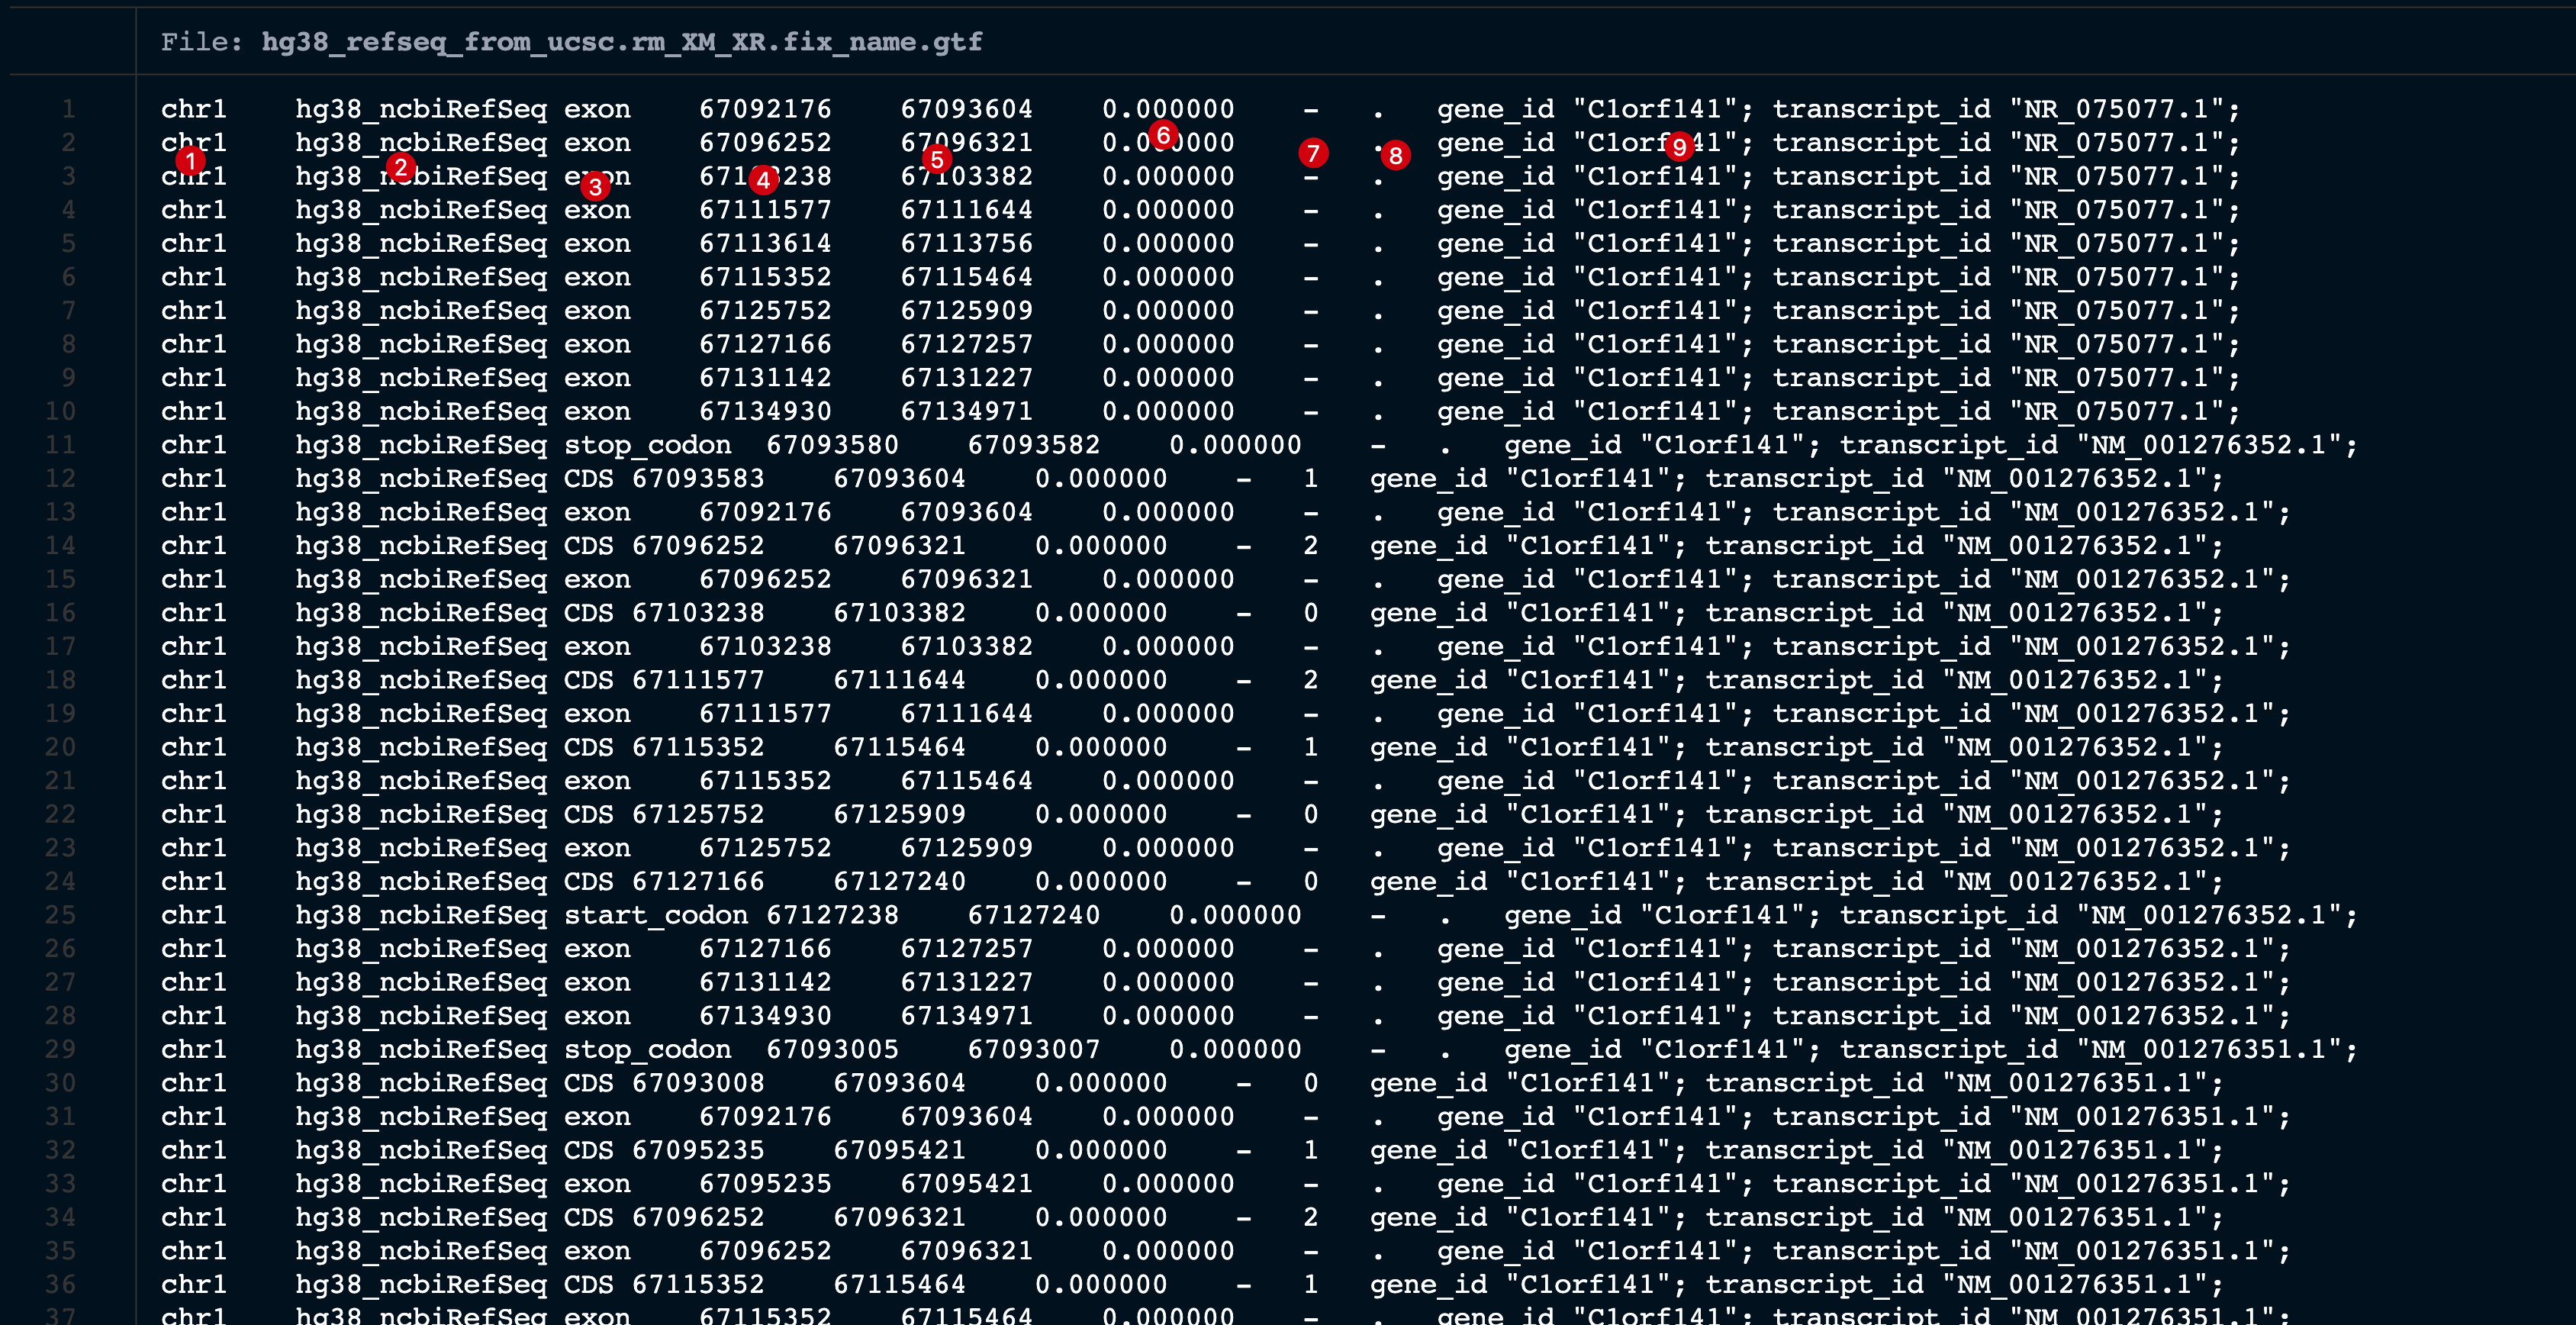
\includegraphics[width=\linewidth]{Images/gtf.png}
    \end{figure}
\end{frame}
\begin{frame}{Demo: another GTF}
    \begin{figure}
        \centering
        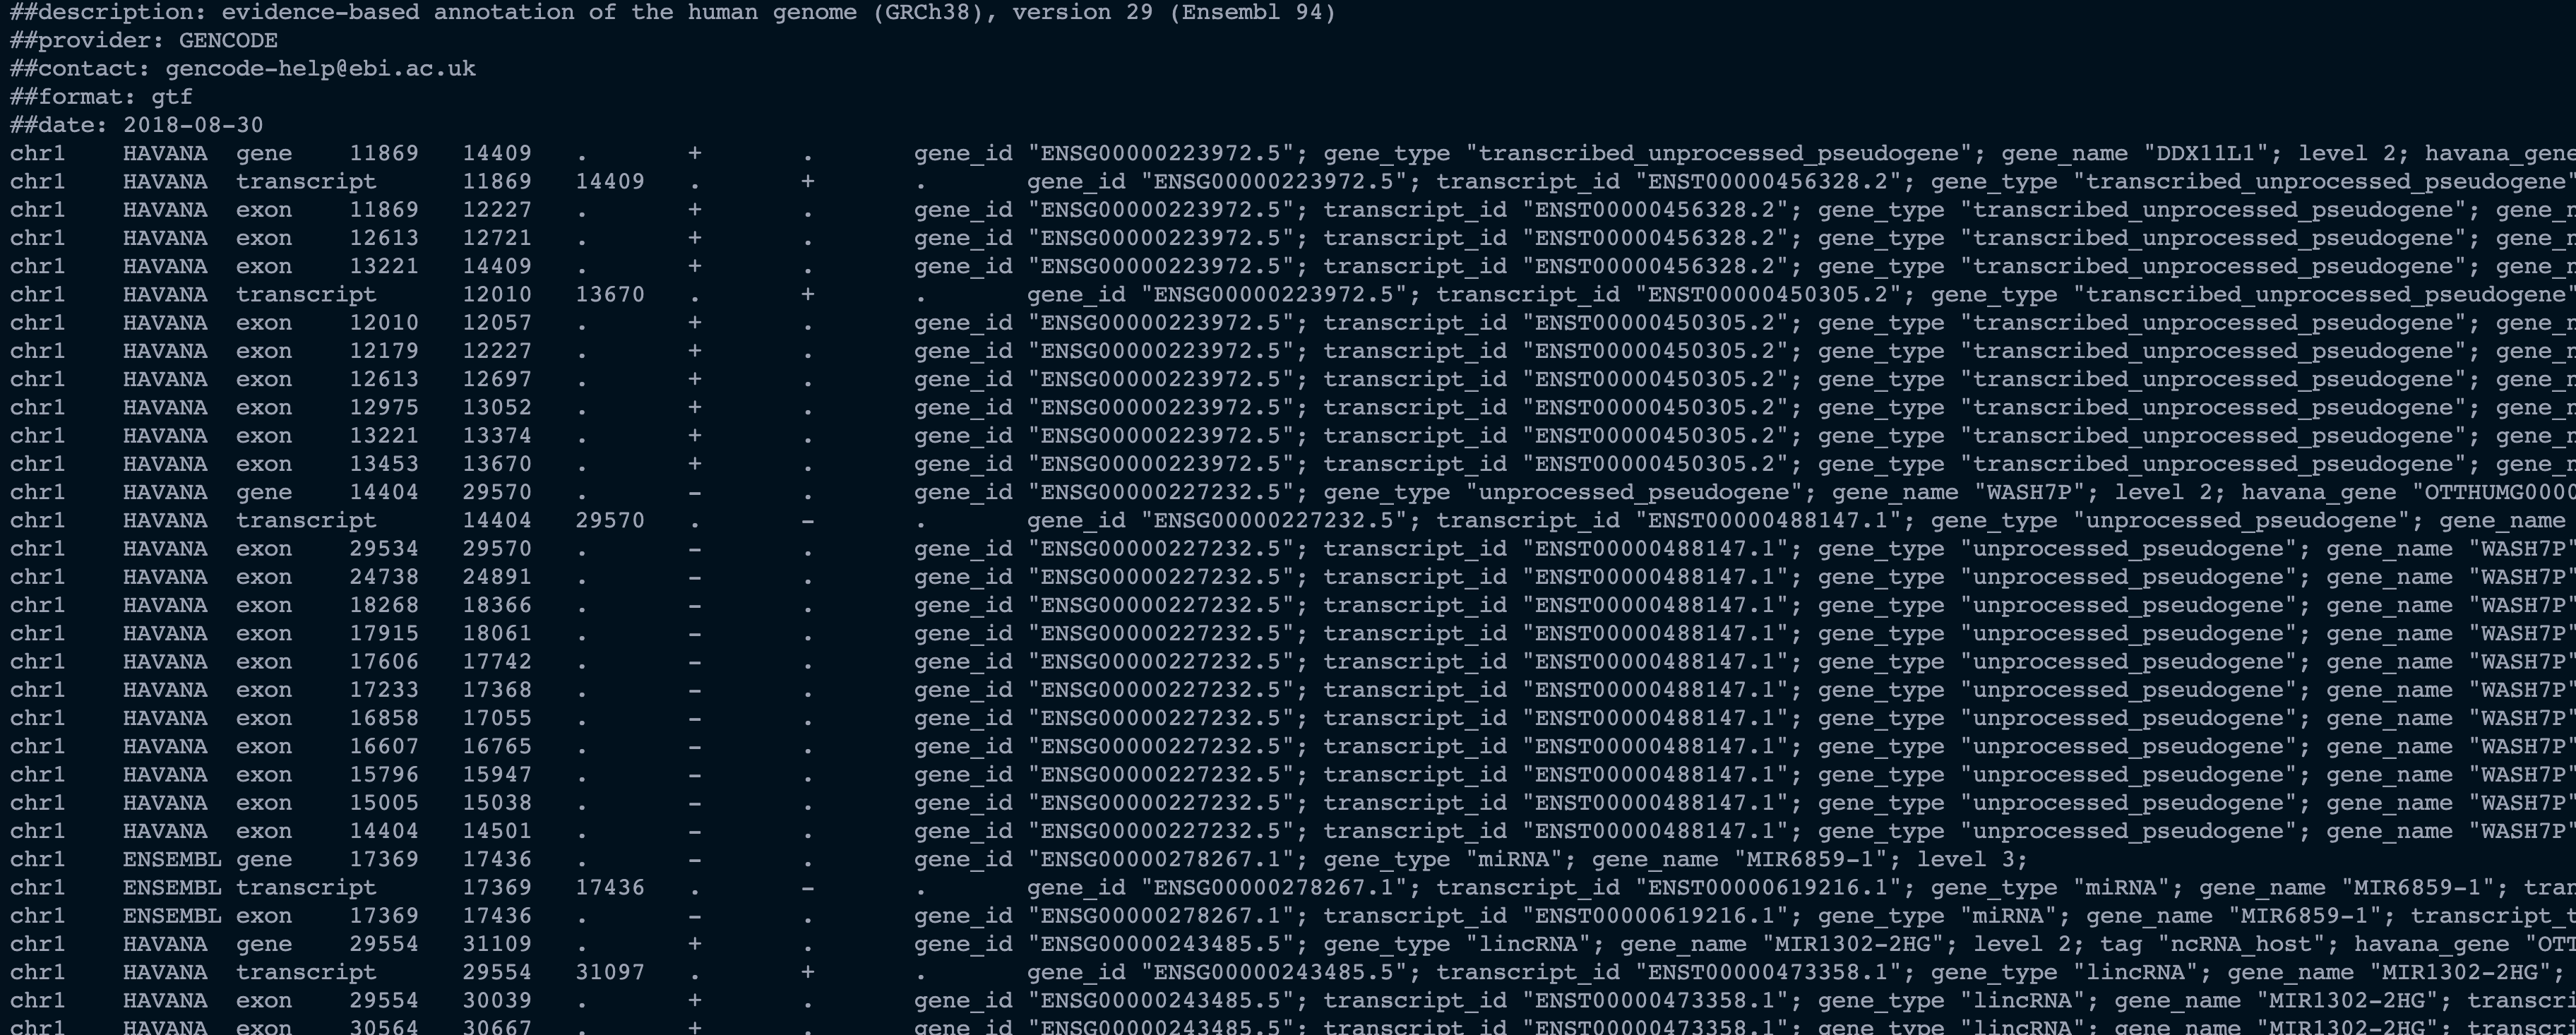
\includegraphics[width=\linewidth]{Images/gtf2.png}
    \end{figure}
\end{frame}

\begin{frame}{Demo: GFF3}
    \begin{figure}
        \centering
        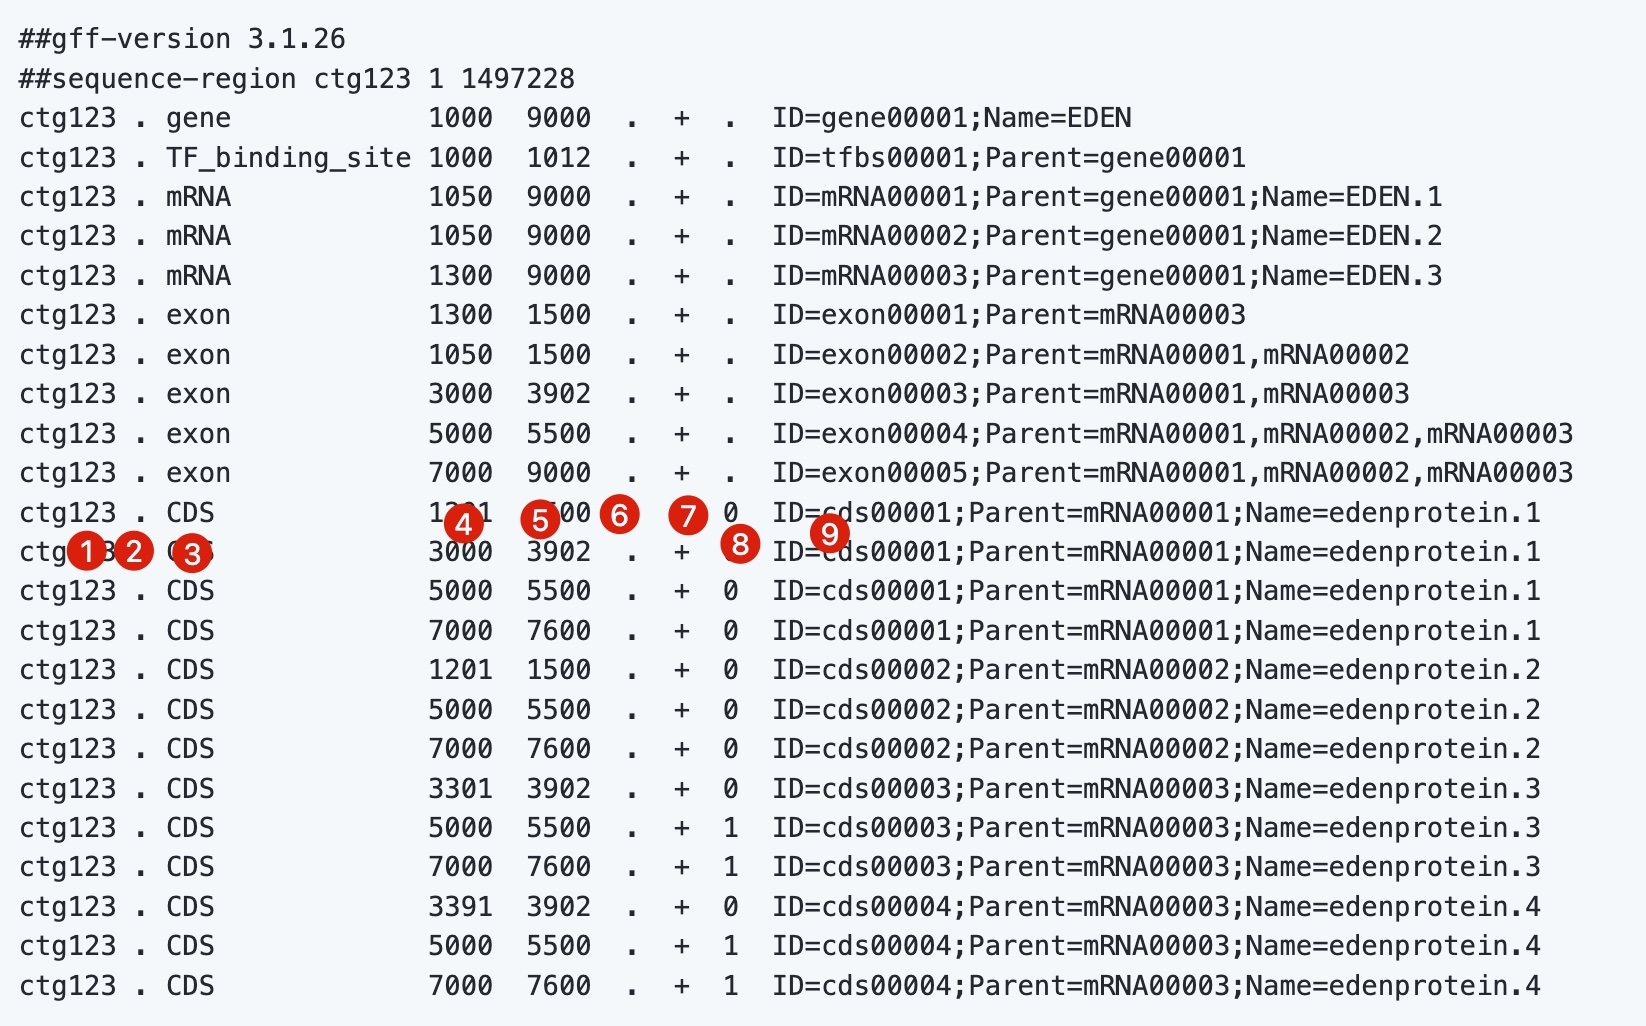
\includegraphics[width=\linewidth]{Images/gff.jpg}
    \end{figure}
\end{frame}


\begin{frame}{Info: 以GTF为例}
    \begin{myoutline}
        \1 1. seq\_id
            \2 序列的编号, 一般为chr或者scanfold编号, 每条染色体拥有一个唯一的ID。
        \1 2. source
            \2 注释的来源, 代表基因结构的来源,可以是数据库的名称,比如来自RefSeq数据库,也可以是软件的名称,比如用GeneScan软件预测得到,当然,也可以为空,用``.''点号填充。
        \1 3. type
            \2 代表区间对应的特征类型, 在GTF中, 常见的类型如下:
                \3 Gene, cDNA, mRNA, 5UTR, 3UTR, exon, CDS, start\_codon, stop\_codon
        \1 4. start
            \2 该基因或转录本在参考序列上的起始位置。
        \1 5. end
            \2 该基因或转录本在参考序列上的终止位置。
        \1 6. score
            \2 得分, 软件提供了统计值, 是注释信息可能性的说明, 可以是序列相似性比对时的E-values值或者基因预测是的P-values值
            \2 ``.''表示为空。
        \1 7. strand
            \2 代表正负链的信息,+表示正链,-表示负链,?表示不清楚正负链的信息
            \2 当正负链信息没有意义时,可以用``.''填充。
    \end{myoutline}
\end{frame}
\begin{frame}{Info: 以GTF为例}
    \begin{myoutline}
        \1 8. phase
            \2 仅对注释类型为``CDS''有效,表示起始编码的位置,有效值为0、1、2
                \3 对于编码蛋白质的CDS来说, 本列指定下一个密码子开始的位置。每3个核苷酸翻译一个氨基酸, 从0开始, CDS的起始位置, 除以3, 余数就是这个值, 表示到达下一个密码子需要跳过的碱基个数。
                \3 0表示该编码框的第一个密码子第一个碱基位于其5'末端
                \3 1表示该编码框的第一个密码子的第一个碱基位于该编码区外
                \3 2表示该编码框的第一个密码子的第一、二个碱基位于该编码区外
            \2 如果\textcolor{red}{Feature为CDS时,必须指明具体值}!
        \1 9. attributes (\textcolor{blue}{更正!})
            \2 一个包含众多属性的列表
                \3 GFF3: 格式为``标签=值'' | ``(tag=value)'', 如果一个序列元件没有Parent属性,说明他的父元件就是scaffold或者chromosome
                \3 GTF: 格式为``标签 值;'' | ``tag value;'',每个特征之后都要有分号(\textcolor{red}{包括最后一个特征})
                \3 GTF: 其内容\textcolor{red}{必须包括gene\_id和transcript\_id}, 其value可以为空``''
    \end{myoutline}
\end{frame}




\begin{frame}[fragile]{GTF和GFF文件操作}
    \begin{columns}
        \column{0.5\textwidth}
        \begin{myoutline}
            \1 ensembl 示例文件下载
                \2 https://www.ensembl.org/
                \2 All genomes (Search 下方)
                \2 选择 Human
                \2 Gene annotation
                \2 Download GTF or GFF3 files for genes, cDNAs, ncRNA, proteins
        \end{myoutline}
        \column{0.5\textwidth}
        \begin{figure}
            \centering
            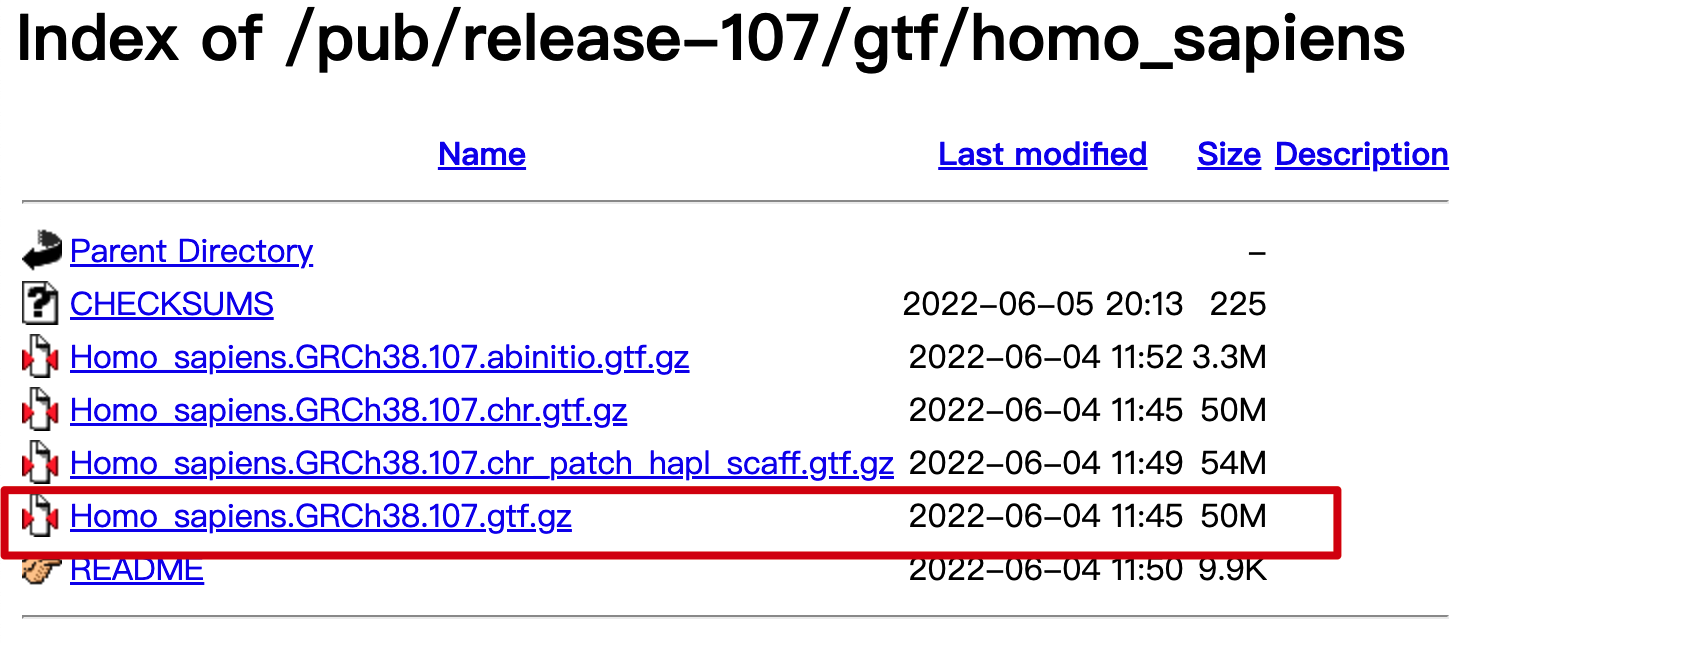
\includegraphics[width=\linewidth]{Images/gtf_download.png}
        \end{figure}
    \end{columns}
    \footnotenoindex{https://www.ensembl.org/}
\end{frame}